\documentclass[a4,12pt]{article}

%--- Packages génériques ---%

\usepackage[english]{babel}
\usepackage[utf8]{inputenc}
\usepackage[T1]{fontenc}
\usepackage[babel=true]{csquotes}
\usepackage{amsmath}
\usepackage{amssymb}
\usepackage{textcomp}
\usepackage{float}
\usepackage{graphicx}
\usepackage{caption}
\usepackage{hyperref}
\usepackage{empheq}
\usepackage{color}
\usepackage{cancel}
\usepackage{textcomp} %% pour les intervalles d'entiers(doubles barres)

%--- Structure de la page ---%

\usepackage{fancyheadings}

\topmargin -1.5 cm
\oddsidemargin -0.5 cm
\evensidemargin -0.5 cm
\textwidth 17 cm
\setlength{\headwidth}{\textwidth}
\textheight 24 cm
\pagestyle{fancy}
\lhead[\fancyplain{}{\thepage}]{\fancyplain{}{\sl MSIAM 3A}}
\chead[\fancyplain{}{{\sl }}]{\fancyplain{}{{Summary}}}
\rhead[\fancyplain{}{}]{\fancyplain{}{Rakotonarivo \& Mazouth--Laurol}}
\lfoot{\fancyplain{}{}}
\cfoot{\fancyplain{}{}}
\cfoot{\thepage }
\rfoot{\fancyplain{}{}}

%--- Raccourcis commande ---%

\newcommand{\R}{\mathbb{R}}
\newcommand{\N}{\mathbb{N}}
\newcommand{\A}{\mathbf{A}}
\newcommand{\B}{\mathbf{B}}
\newcommand{\C}{\mathbf{C}}
\newcommand{\D}{\mathbf{D}}
\newcommand{\ub}{\mathbf{u}}

\DeclareMathOperator{\e}{e}
%--- Header to write code ---%
\usepackage { listings }
%%configuration de listings
\lstset{
	language=c++,
	basicstyle=\ttfamily\small, %
	identifierstyle=\color{black}, %
	keywordstyle=\color{blue}, %
	stringstyle=\color{black!60}, %
	commentstyle=\it\color{green!95!yellow!1}, %
	columns=flexible, %
	tabsize=2, %
	extendedchars=true, %
	showspaces=false, %
	showstringspaces=false, %
	numbers=left, %
	numberstyle=\tiny, %
	breaklines=true, %
	breakautoindent=true, %
	captionpos=b
}


\usepackage{xcolor}


\definecolor{Zgris}{rgb}{0.87,0.85,0.85}


\newsavebox{\BBbox}
\newenvironment{DDbox}[1]{
	\begin{lrbox}{\BBbox}\begin{minipage}{\linewidth}}
		{\end{minipage}\end{lrbox}\noindent\colorbox{Zgris}{\usebox{\BBbox}} \\
	[.5cm]}
%--- Mode correction et incréments automatiques ---%

\usepackage{framed}
\usepackage{ifthen}
\usepackage{comment}

\newcounter{Nbquestion}

\newcommand*\question{%
\stepcounter{Nbquestion}%
\textbf{Question \theNbquestion. }}

\newboolean{enseignant}
%\setboolean{enseignant}{true}
\setboolean{enseignant}{false}

\ifthenelse{
\boolean{enseignant}}{
\newenvironment{correction}{\begin{shaded}}{\end{shaded}}
}
{
\excludecomment{correction}
}

%%%%%%%%%%%%%%%%%%%%%%%%%%%%%%%%%%%%%%%%%%%%%%%%%%%%%%%%
% 							               EN-TETE        

\title{\textbf{Tomography reconstruction from 2D projections}}
\author{
\begin{tabular}{cc}
	\textsc{Rakotonarivo Michi} & \textsc{Maxime Mazouth--Laurol}
\end{tabular}}   
\date{\small $11^{th}$ December 2017}

\makeatletter
	\def\thetitle{\@title}
	\def\theauthor{\@author}
	\def\thedate{\@date}
\makeatother 

\usepackage{etoolbox}
\usepackage{titling}
\setlength{\droptitle}{-7em}

\setlength{\parindent}{0cm}

\makeatletter
% patch pour le bug concernant les parenthèses fermantes d'après http://tex.stackexchange.com/q/69472
\patchcmd{\lsthk@SelectCharTable}{%
  \lst@ifbreaklines\lst@Def{`)}{\lst@breakProcessOther)}\fi}{}{}{}
\begin{document}

\maketitle
\section{Define the frame of work}
~~ For any computer project, a frame of work must be defined. As this project is all about medical imagery made of disks of various intensities, the idea of creating three main classes defining images came naturally. 
\paragraph{Framework class} 
This class sets up the area where projections will be taken into account. For convenience, a disk has been preferred, the idea being to be able to translate the center and change the radius(e.g to compute only subsections of an image). Plus, it contains a list of images, so that we can handle them easily, whether it is switching between images, adding or removing them.
\begin{itemize}
\item \textbf{Attributes}
	\begin{itemize}
	\item center = [Xcenter,Ycenter]
	\item radius
	\item imageList
	\item currentImage
	\end{itemize}
	
\item \textbf{Methods}
	\begin{itemize}
	\item setters and getters for above attributes
	\item addition and removal of an image
	\item plot the framework and the current image
	\end{itemize}
\end{itemize}

\paragraph{Image class}
In the scope of the project, an image is nothing but a set of disks with different sizes and intensities. Thus, the class takes as an attribute the list of such disks, with the possibility to access it, to add or remove disks from the list.

\paragraph{Disk class}
It contains a center, a radius and a constant intensity corresponding to the attenuation function. 

\section{Derive the sinogram of a given image}
After establishing the statements given in the previous section, the first step of the image reconstruction process is the computation of projection $\Re$ over every angle $\phi \in [0,2\pi]$, leading to a sinogram. Here a presented a few properties to be used for this purpose.

\subsection{Mathematical results}
\subsubsection{Projection on a line}
Let's remind the Radon Transform formula:
\[
p(\phi,s) = \Re f(\phi,s) = \int_{-\infty}^{+\infty}f(s\theta_{\phi} + l\sigma_{\phi})dl
\]
In our case, for a given image $I$, computing the projection gives:
\[
p(\phi,s) = \int_{disk = 0}^{N}length(disk,line(\phi,s))*disk.intensity, \text{with N = Card(I) \\}
\] 
using the linearity of the radon Transform operator and the fact that, for a single disk, the intensity(corresponding to $f$) is constant.

\subsubsection{Dilatation of the Radon Transform}
Let's define $D \in \mathbb{R}$,
\[
	f_{D}(x) = f(\frac{x}{D})
\]
For any scaling coefficient $D$, the following formula can be derived : 
\[
\Re f_{D}(\phi,s) = D\Re f(\phi,\frac{s}{D})
\]
It numerically means that, for any disk centered in $[0,0]$, its radon Transform can be obtained from the unit disk radon Transform.

\subsubsection{Translation of the Radon Transform}
Let's define $a \in \mathbb{R}^{n}$ such that, 
\[
	f_{a}(x) = f(x-a)
\]
For any translation vector $a$, we have :
\[
\Re f_{a}(\phi,s) = \Re f(\phi,x.a)
\]
Hence, the radon Transform of a non-centered disk can be derived from the projection of the centered disk. \\ \\

~~ Finally, computing numerically the radon transform of any disk can be reduced to a computation on the unit disk centered in $[0,0]$. 
\subsection{Numerical results}
\begin{figure}[h!]
   \begin{minipage}[c]{.46\linewidth}
      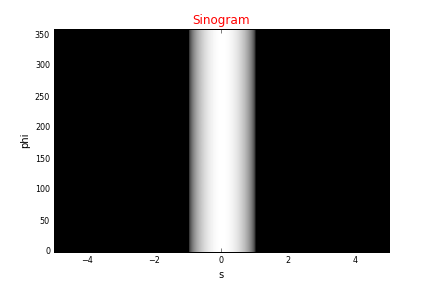
\includegraphics[scale=0.5]{../images/sinograms/unitDisk.png} 
      \captionof{figure}{Unit disk}
   \end{minipage} \hfill
   \begin{minipage}[c]{.46\linewidth}
      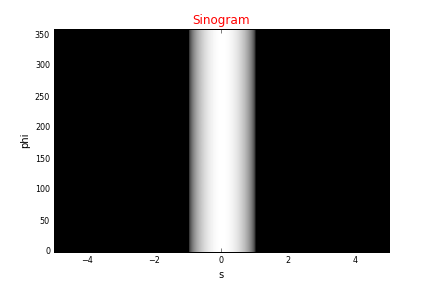
\includegraphics[scale=0.5]{../images/sinograms/centeredDisk2.png} 
      \captionof{figure}{Centered disk, $r=2$}
   \end{minipage}
\end{figure}

The simplest case to ensure the correctness of our implementation is the unit disk. As it is symmetric to any centered axis, the computed projection must be independent of the angle $\phi$, which is exactly what is obtained for Figure 1. In Figure 2, the disk has the same intensity and center, but the radius is 2.  \\
\section{Study of the moments}
For now, moments have been computed only for the simplest cases : sets of centered disks. Still, we get consistent results, as the moment is supposed to be constant over $\phi$.
\subsection{Moments from sinograms}
\begin{figure}[h!]
   \begin{minipage}[c]{.46\linewidth}
      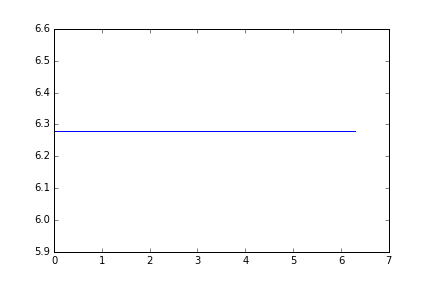
\includegraphics[scale=0.5]{../images/moments/unitDiskMoment0.png} 
      \captionof{figure}{order 0 for Unit disk}
   \end{minipage} \hfill
   \begin{minipage}[c]{.46\linewidth}
      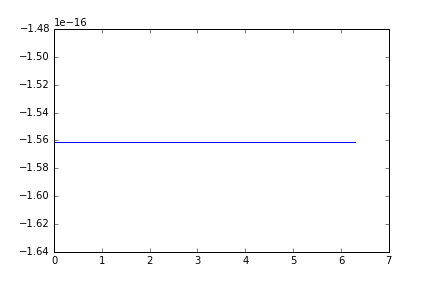
\includegraphics[scale=0.5]{../images/moments/unitDiskMoment1.png}  
      \captionof{figure}{order 1 for Unit disk}
   \end{minipage}
\end{figure}
\begin{figure}[h!]
   \begin{minipage}[c]{.46\linewidth}
      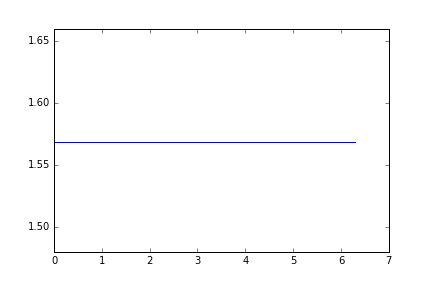
\includegraphics[scale=0.5]{../images/moments/unitDiskMoment2.png} 
      \captionof{figure}{order 2 for Unit disk}
   \end{minipage} \hfill
   \begin{minipage}[c]{.46\linewidth}
      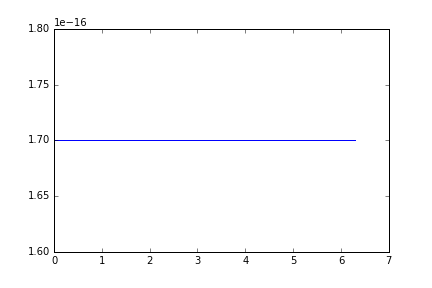
\includegraphics[scale=0.5]{../images/moments/unitDiskMoment3.png} 
      \captionof{figure}{order 3 for Unit disk}
   \end{minipage}
\end{figure}
\subsection{Projections on trigonometric polynomial basis}
We have shown in class that, $\forall n \in \mathbb{N}, \exists {a_i} \text{ and } {b_i} \text{ coefficients,}         $
\[
	M_{n}(\phi) = \displaystyle \sum_{i=0}^{\lceil \frac{n}{2} \rceil}a_{i}cos((n-2i)\phi) + b_{i}sin((n-2i)\phi)
\]
\begin{figure}[h!]
   \begin{minipage}[c]{.46\linewidth}
      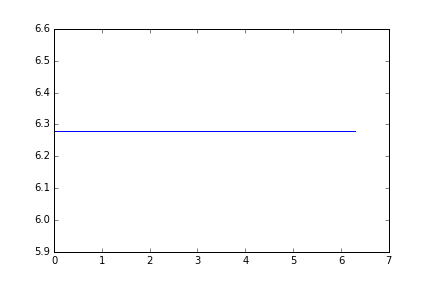
\includegraphics[scale=0.5]{../images/moments/unitDiskProjMoment0.png} 
      \captionof{figure}{order 0 for Unit disk}
   \end{minipage} \hfill
   \begin{minipage}[c]{.46\linewidth}
      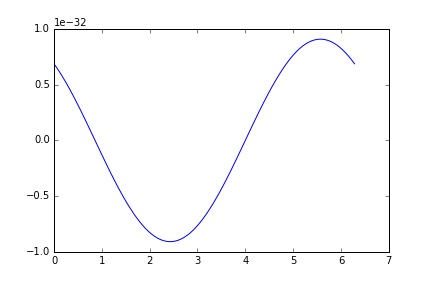
\includegraphics[scale=0.5]{../images/moments/unitDiskProjMoment1.png}  
      \captionof{figure}{order 1 for Unit disk}
   \end{minipage}
\end{figure}
\begin{figure}[h!]
   \begin{minipage}[c]{.46\linewidth}
      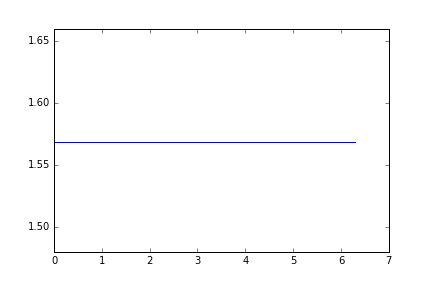
\includegraphics[scale=0.5]{../images/moments/unitDiskProjMoment2.png} 
      \captionof{figure}{order 2 for Unit disk}
   \end{minipage} \hfill
   \begin{minipage}[c]{.46\linewidth}
      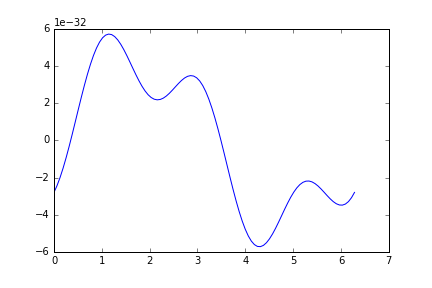
\includegraphics[scale=0.5]{../images/moments/unitDiskProjMoment3.png} 
      \captionof{figure}{order 3 for Unit disk}
   \end{minipage}
\end{figure}

The numerical values have not been checked yet, but the results look like sums of $\cos$ and $\sin$ functions.
\end{document}